\Chapter{Project Implementation}

The GradeBadge application is designed to work on mobile, tablet devices and desktop computers. The UI of the application is developed using Bootstrap. When a page requires the data to be loaded from server or modified or deleted, a request is sent to the Web server over  HTTPS. The requests are sent to the Web server using Ajax. For handling Ajax requests and responses, this application uses JQuery Ajax API. All UI components are dynamically created or initialized in response to the data received from the Web server.

\newpage
\section{Loading Screen}
When the GradeBoard application is loaded, a loading screen is presented to the user as shown in the Figure ~\ref{fig:loading_screen}. The loading screen shows application logo and loading progess bar, and the screen is automatically redirected after the loading completed. 

\vspace{3em}
\begin{figure}[H]
\begin{center}

\includegraphics[height=3.8in,width=6.5in]{images/loading-screen.jpg}
\caption{GradeBadge Loading Screen}
\label{fig:loading_screen}
\end{center}
\end{figure}

\newpage
\section{Login Screen}
GradeBadge uses Facebook account for users to login. When the user is not logged-in to Facebook, the screen is automatically redirected to the Facebook login screen as shown in Figure~\ref{fig:login_screen}. Every user in the system can be badge issuer and badge earner.

\vspace{3em}
\begin{figure}[H]
\begin{center}
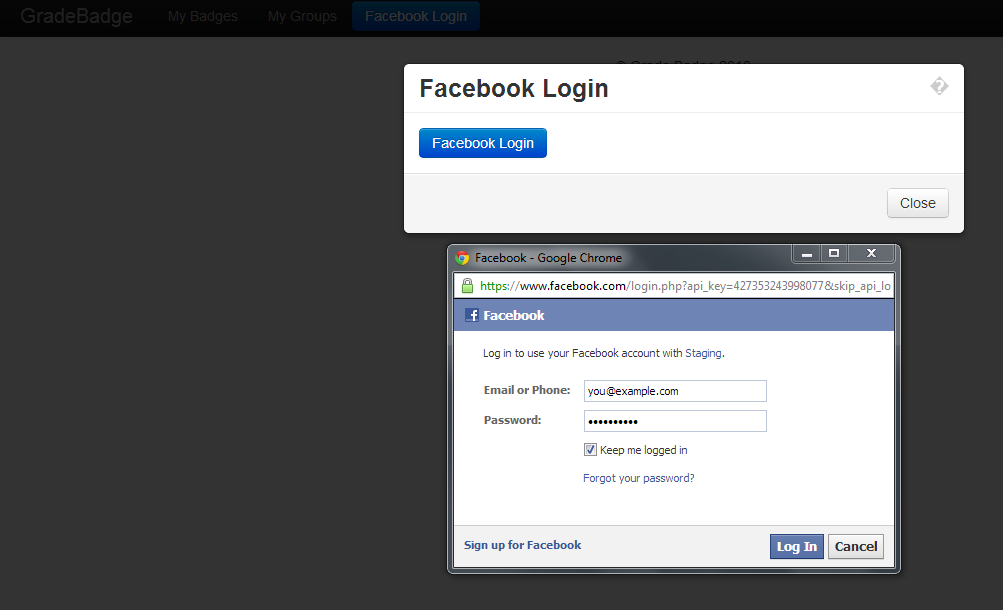
\includegraphics[height=6.8in,width=6.5in]{images/facebook-login.jpg}
\caption{GradeBadge Login Screen}
\label{fig:login_screen}
\end{center}
\end{figure}

\newpage
\section{Group Page}
 as shown in Figure~\ref{fig:group-page1}. 

\vspace{3em}
\begin{figure}[H]
\begin{center}

\includegraphics[height=3.8in,width=6.5in]{images/group-page1.png}
\caption{GradeBadge Group Page}
\label{fig:group-page1}
\end{center}
\end{figure}

\newpage
\section{Add New Group Page}
 as shown in Figure~\ref{fig:add-new-group}. 

\vspace{3em}
\begin{figure}[H]
\begin{center}
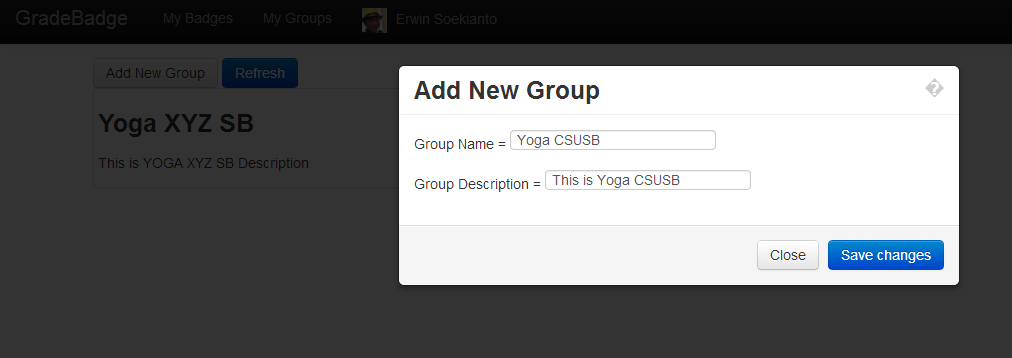
\includegraphics[height=3.8in,width=6.5in]{images/add-new-group.png}
\caption{GradeBadge Add New Group Page}
\label{fig:add-new-group}
\end{center}
\end{figure}

\newpage
\section{Group Page}
 as shown in Figure~\ref{fig:group-page2}. 

\vspace{3em}
\begin{figure}[H]
\begin{center}

\includegraphics[height=3.8in,width=6.5in]{images/group-page2.png}
\caption{GradeBadge Group Page Added}
\label{fig:group-page2}
\end{center}
\end{figure}


